\section{Normal Distribution}
\label{sec:Normal Distribution}

\subsection{Objective}
Using the Gaussian random numbers we find the mean and variance. 

\subsection{Theory}
The normal distribution or the Gaussian distribution is a continuous probability distribution 
shaped like a bell curve. It is defined by two parameters, mean($\mu$) and variance($\sigma^2$).
The probability density function is given by:

\begin{equation}
	f(x) = \frac{1}{\sqrt{2\pi\sigma^2}} e^{-\frac{(x-\mu)^2}{2\sigma^2}}
\end{equation}

\pagebreak
\subsection{Matlab Code}

\inputminted[fontsize=\footnotesize,autogobble]{matlab}{code/density.m}

\subsection{Output}

\begin{figure}[!htb]
	\centering
	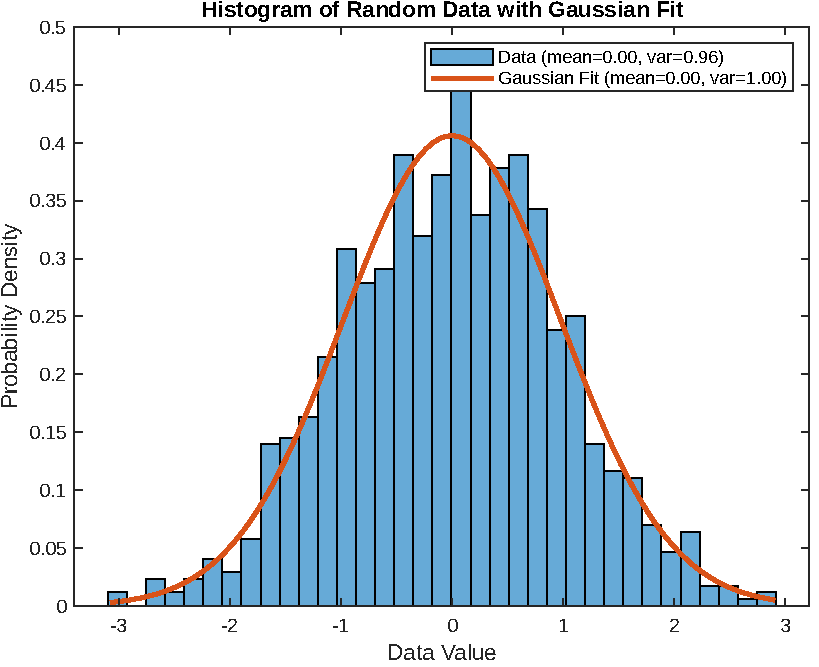
\includegraphics[width=0.6\textwidth]{res/figures/Figure_2.pdf}
	\label{output:gaussian distribution}
	\caption{Gaussian Distribution}
\end{figure}